\documentclass{article}

\usepackage{amsmath}
\usepackage{amsthm}
\usepackage{amssymb}
\usepackage{mathtools}
\usepackage{enumerate}
\usepackage{lipsum}
\usepackage{multicol}
\usepackage{graphicx}

\renewcommand{\thefootnote}{\fnsymbol{footnote}}

\title{Analysuppgift 3 - Analys av kurva}
\author{Emma Bastås}
\date{November 6, 2022}

\begin{document}

\maketitle

\noindent Uppgiften är att till kurvan $y = f(x)$ där:

\begin{gather*}
  f(x) = \frac{|x-1| + 2x^{2}}{x + 1}
\end{gather*}
\\
bestämma lokala och globala extrempunkter och asymptoter samt rita grafen.
\\
\\
Vi börjar med att att falluppdela $f(x)$ och därefter förenkla uttrycken med polynomdivision:

\begin{align}
  f(x) &=
         \begin{cases}
           \begin{aligned}[t]
             & \frac{x - 1 + 2x^{2}}{x+1} & \text{om} \; x \geq 1 \\
             & \frac{-x + 1 +2x^{2}}{x+1} & \text{om} \; x < 1
           \end{aligned}
         \end{cases} \notag \\[4pt]
       & =
         \begin{cases}
           \begin{aligned}[t]
             & 2x - 1 & \text{om} \; x \geq 1 \\
             & 2x - 3 + \frac{4}{x + 1} & \text{om} \; x < 1
          \end{aligned}
         \end{cases}\text{.} \label{cases}
\end{align}


\subsection*{Asymptoter}

Det finns tre typer av asymptoter att söka efter:

\begin{itemize}
        \item \textbf{Vertikal asymptot}. Linjen $x = a$ är en vertikal asymptot till $y = f(x)$ om $\lim_{x \to a}f(x) = \pm\infty$.
        \item \textbf{Horisontell asymptot}. Linjen $y = a$ är en horisontell asymptot till $y = f(x)$ om $\lim_{x \to \pm\infty}f(x) = a$.
        \item \textbf{Sned asymptot}. Linjen $y = kx + m$ där $k \neq 0$ är en sned asymptot till $y = f(x)$ om $\lim_{x \to \pm\infty}[f(x) - (kx +m)] = 0$.
\end{itemize}

\noindent Det finns en punkt då $f(x)$ går mot oändligheten, och den ligger i $x = -1$. Detta är den enda vertikala asymptoten till $y = f(x)$.
\\
\\
Vi testar om $f(x)$ har en horisontell asymptot då $x$ går mot $+\infty$:

\begin{align*}
  & \lim_{x \to +\infty}f(x) = L\\
  \iff \quad & \lim_{x \to +\infty}[2x - 1] = L\text{.}
\end{align*}
\\
Vi ser direkt att detta saknar gränsvärde och att en horisontell asymptot är utesluten. Vi testar nu om det finns en sned asymptot istället:

\begin{align*}
  & \lim_{x \to +\infty}[f(x) - (kx + m)] = 0\\
  \iff \quad & \lim_{x \to +\infty}[2x - 1 - (kx + m)] = 0\\
  \iff \quad & \lim_{x \to +\infty}[(2 - k)x - (m + 1)] = 0\\
  \iff \quad & k = 2 \quad \text{och} \quad m = -1\text{.}
\end{align*}
\\
Vi ser att linjen $y = 2x - 1$ är en sned asymptot till $y = f(x)$. På liknande sätt finner vi att linjen $y = 2x -3$ är en sned asymptot då $x$ går mot $-\infty$.
\\
\\
Nu har vi funnit samtliga asymptoter till $y = f(x)$: $x = -1$, $y = 2x -1$ och $y = 2x - 3$.


\subsection*{Extrempunkter}

\noindent Vi bestämmer derivatan $f'(x)$ till $f(x)$ genom att derivera fallen separat:

\begin{gather*}
  \text{(\ref{cases})} \implies f'(x) =
  \begin{cases}
    \begin{aligned}[t]
      & 2 & \text{om} \; x > 1 \\
      & 2 - \frac{4}{(x + 1)^{2}} & \text{om} \; x < 1
    \end{aligned}
  \end{cases}\text{.}
\end{gather*}
\\
Notera att $f(x)$ inte är deriverbar i punkten $x = 1$. Går vi tillbaka till derivatans definition finner vi att vi får två olika derivator beroende på från vilket håll vi närmar oss $x = 1$, en egenskap som gör derivatan odefinierad i den punkten.
\\
\\
Att en punkt $x_{0}$ är ett extremvärde till en funktion $f(x)$ medför alltid att ett av tre påståenden är sant:

\begin{enumerate}[i)]
        \item $x_{0}$ är en ändpunkt i definitionsintervallet till $f(x)$.
        \item $f(x)$ är diskontinuerlig i $x_{0}$.
        \item $f(x)$ är deriverbar i $x_{0}$ och $f'(x_{0}) = 0$.
\end{enumerate}

\noindent I vårt fall är $f(x)$ definierad i intervallen $x < -1$ och $x > -1$. Således kan aldrig det första påståendet vara sant. Vi vet också att $f(x)$ är kontinuerlig i hela sin definitionsmängd, således kan aldrig det andra påståendet vara sant. Det lämnar oss med det sista påståendet, alla extrempunkter till $f(x)$ är nollställen till $f'(x)$.
\\
\\
Vi finner dessa nollställen. För $x > 1$ är $f'(x) = 2$ och detta saknar nollställen, för fallet $x < 1$ ställer vi upp och löser ekvationen:

\begin{align*}
  & f'(x) = 0 \quad x < 1 \\
  \iff \quad & 2 - \frac{4}{(x + 1)^{2}} = 0 \text{.} \\
  \iff \quad & 2(x + 1)^{2} - 4 = 0 \\
  %\iff \quad & (x + 1)^{2} = 2 \\
  %\iff \quad & x + 1 = \pm \sqrt{2} \\
  \iff \quad & x = -1 \pm \sqrt{2}\text{.}
\end{align*}
\\
Vi finner även de intervall för vilket $f'(x) < 0$, detta är nödvändigt för att senare avgöra om nollställena är max- eller minimipunkter eller terrasspunkter.

\begin{align}
  & f'(x) < 0 \notag \\
  \iff \quad &
  \begin{aligned}
    \begin{cases}
      2 < 0 & \text{då} \; x > 1 \\
      2 - \frac{4}{(x+1)^{2}} < 0 & \text{då} \; x < 1
    \end{cases}
  \end{aligned}\text{.} \label{fp_cases}
\end{align}
\\
Det första fallet är alltid falskt och kan därför förkastas:

\begin{align}
  \text{(\ref{fp_cases})} \quad \iff \quad & 2 - \frac{4}{(x+1)^{2}} < 0 \quad \text{och} \quad x < 1\text{.} \label{fp_nocase}
\end{align}
\\
Nämnaren $(x + 1)^{2}$ är strikt större än noll för alla värden av $x$ i definitionsmängden till $f'(x)$ och vi kan därför multiplicera båda led i olikheten med nämnaren:

\begin{align}
  \text{(\ref{fp_nocase})} \quad \iff \quad & 2(x + 1)^{2} - 4 < 0 & \text{och} \quad x < 1 \notag \\
  \iff \quad & (x + 1)^{2} < 2 & \text{och} \quad x < 1\text{.} \label{fp_square}
\end{align}
\\
Nu drar vi kvadratroten ur båda led och det är här viktigt att komma ihåg att $\sqrt{a^{2}} \neq a\,$! Istället är det $\sqrt{a^{2}} = |a|$ som är den korrekta identitet.

\begin{align*}
  \text{(\ref{fp_square})} \quad \iff \quad & |x + 1| < \sqrt{2} & \text{och} \quad x < 1 \\
  \iff \quad &
               \begin{aligned}
                 \begin{cases}
                   x + 1 < \sqrt{2} & \text{då} \; x > - 1 \\
                   -x -1 < \sqrt{2} & \text{då} \; x < - 1
                 \end{cases}
               \end{aligned}
  & \text{och} \quad x < 1\\
  \iff \quad &
              \begin{aligned}
                -1 &< x < \sqrt{2} - 1 \\
                -1 -\sqrt{2} &< x < - 1\text{.}
              \end{aligned}
\end{align*}
\\
Nu vet vi både för vilka värden av $x$ som $f'(x)$ är noll och strikt mindre än noll, och därav vet vi också för vilka $x$ som $f'(x)$ är strikt större än noll, nämligen:

\begin{alignat*}{2}
  & x < -1 - \sqrt{2} &&\quad\text{eller}\\
  & \sqrt{2} - 1 < x < 1 &&\quad\text{eller} \\
  & 1 < x\text{.} &&
\end{alignat*}
\\
Med denna information kan vi besvara frågan om extrempunkter, för att göra det enklare för oss så sammanställer vi relevant data i en tabell:
\\
\\
\begin{tabular}[c]{l | c | c | c | c | c | c | c | c | c}
  $x$     &   & $-\sqrt{2} - 1$ &     & $-1$ &     & $\sqrt{2} - 1$ &     & 1    &     \\ \hline
  $f'(x)$ & + & $0$             & $-$ & odef & $-$ & $0$            & $+$ & odef & $+$ \\
\end{tabular}
\\
\\
\\
Vi ser nu att $x = -\sqrt{2} - 1$ är ett lokalt strikt maximum och att $x = \sqrt{2} - 1$ är ett lokalt strikt minimum. Det finns inga andra extrempunkter utöver dessa. Från avsnittet \textbf{Asymptoter} konstaterade vi att att $y = f(x)$ inte har några horisontella asymptoter, och därav är obegränsad. Vi ser från tabellen att $f(x)$ då är både uppåt och nedåt obegränsad så de två extrempunkter vi funnit är inte globala extrempunkter.

\section*{Grafritning}

Genom att komplettera den tidigare tabellen med ett par beräknade punkter $(x, f(x))$ på kurvan så kan vi skissa upp ett approximerat utseende:
\\
\\
\begin{tabular}[c]{l | c | c | c | c | c | c | c | c | c}
  $x$     &   & $-\sqrt{2} - 1$ &     & $-1$ &     & $\sqrt{2} - 1$ &     & 1    &     \\ \hline
  $f'(x)$ & + & $0$             & $-$ & odef & $-$ & $0$            & $+$ & odef & $+$ \\
  $f(x)$  &   & $-\tfrac{8}{\sqrt{2}} - 5$ &&&     & $\tfrac{8}{\sqrt{2}} - 5$ &&&
\end{tabular}
\\
\\
Det är viktigt att inte blanda ihop de sneda asymptoterna. När kurvan går mot $-\infty$ närmar den sig asymptoten $y = 2x - 3$, och när kurvan går mot $+\infty$ närmar den sig asymptoten $y = 2x - 1$.

\newpage

\noindent Vi approximerar även en del värden som förekommer i tabellen till trevliga bråk:

\begin{gather*}
  \sqrt{2} = \frac{2\sqrt{2}}{2} = \frac{\sqrt{8}}{2} \approx \frac{\sqrt{9}}{2} = \frac{3}{2} \implies\\
  -\sqrt{2} - 1 \approx -\frac{5}{2} \quad \text{och} \quad \sqrt{2} - 1 \approx \frac{1}{2}
\end{gather*}\begin{gather*}
  \frac{8}{\sqrt{2}} = \frac{\sqrt{64}}{\sqrt{2}} = \sqrt{32} \approx \sqrt{36} = 6 \implies\\
  -\frac{8}{\sqrt{2}} - 5 \approx -11 \quad \text{och} \quad \frac{8}{\sqrt{2}} - 5 \approx 1\text{.}
\end{gather*}

Slutligen, den ritade grafen:
\begin{figure}[h]
  \centering
  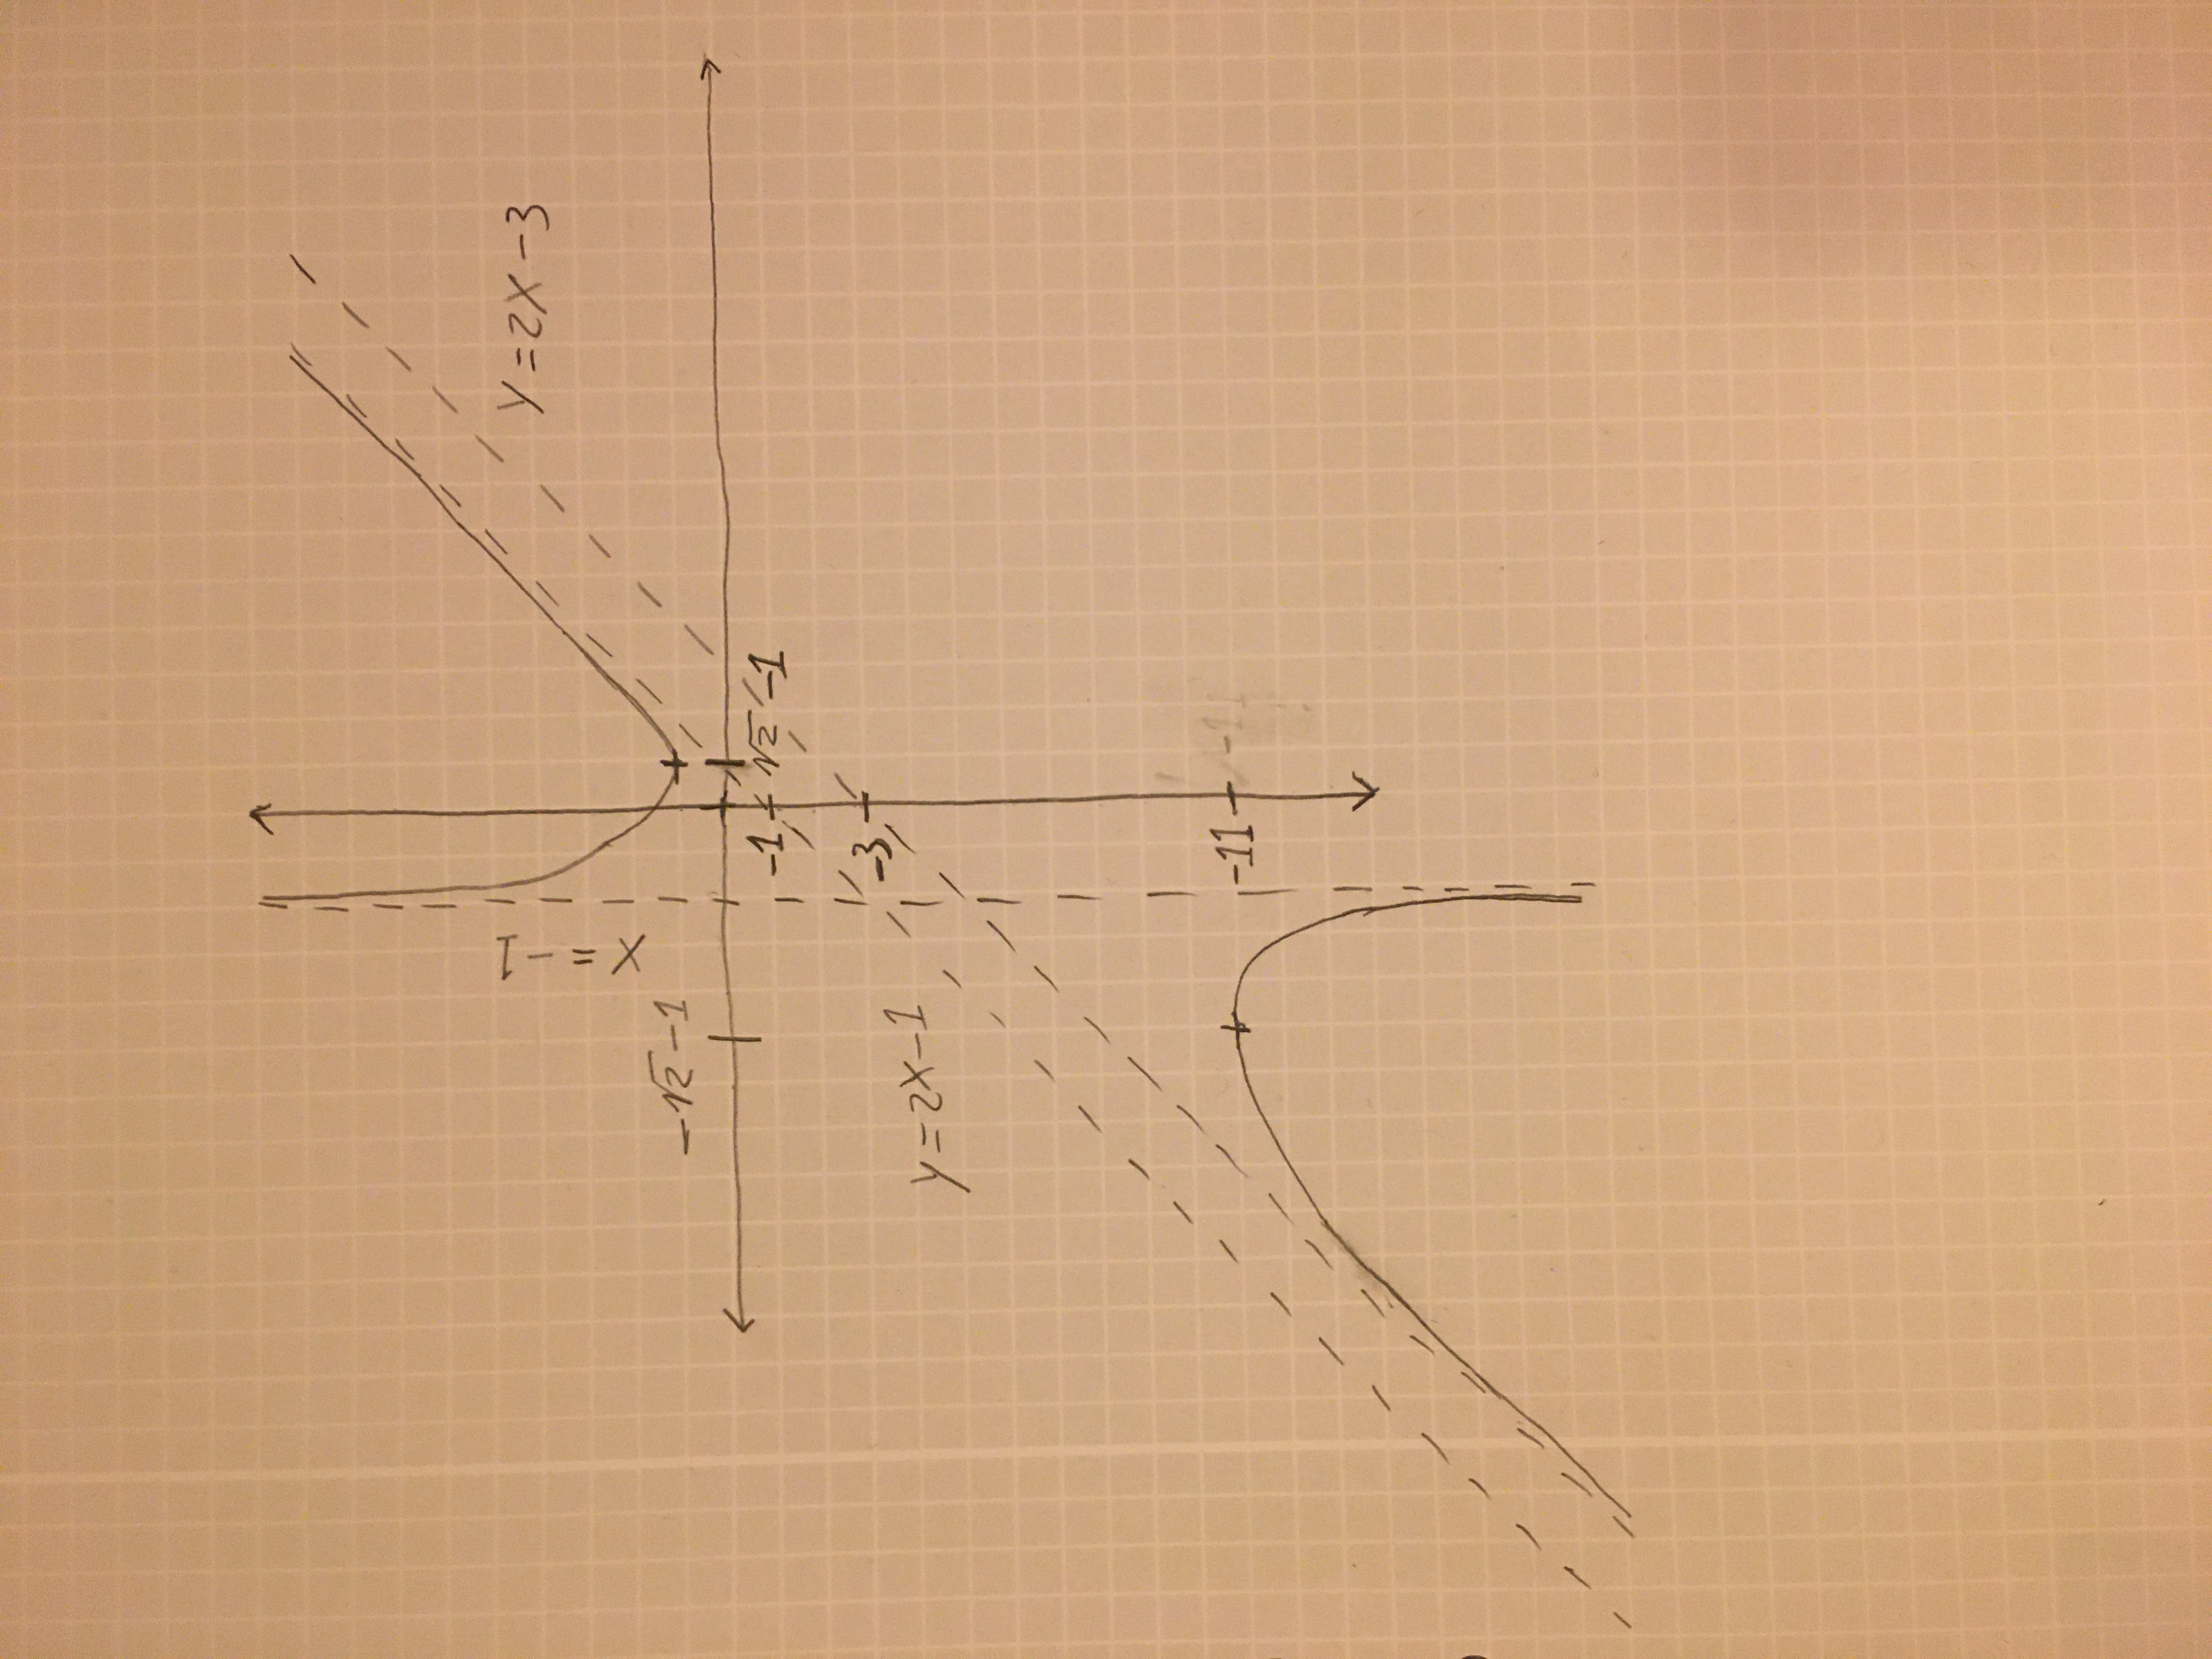
\includegraphics[width=10cm, angle=270]{skiss.jpg}
\end{figure}

\end{document}
